\section{Installation}
\label{cha:Installation}

\subsection{Initial Inspection}
Check the contents of the shipment for completeness and possible transport damage. If the contents are incomplete or damaged, a claim should be filed with the carrier immediately and the DK-Audio Sales or Service organisation should be notified in order to facilitate the repair or replacement of the instrument.

\subsection{Safety Instruction}
\subsubsection{Earthing}
Before any other connection is made, the instrument must be connected to a protective earth conductor in one of the following ways:
\begin{itemize}
\item Via the three-core mains cable
\item Via the protective earth terminal marked 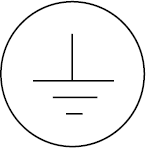
\includegraphics[width=1em]{fig/ground_symbol}
\end{itemize}

Before connecting the equipment to the mains of the building installation, the proper functioning of the protective earth lead of the building installation needs to be verified.

\begin{center}
\fbox{
\parbox{0.95\textwidth}{
\textbf{WARNING}: Any interruption of the protective conductor inside or outside the instrument, or
disconnection of the protective earth terminal, is likely to make the instrument dangerous.
Intentional interruption is prohibited.
}}
\end{center}

\subsubsection{Mains Voltage Cord and Fuses}
Different power cords are available for the various voltage outlets.

\textbf{Note:}
If the mains plug has to be adapted to the local situation it should only be done by a qualified
person.

This instrument is equipped with a tap-less switch mode power supply that covers most nominal
voltage ranges in use: 90-240V AC RMS. This obviates the need to adapt to the local mains voltage.

The mains frequency is 48-65 Hz.

\begin{center}
\fbox{
\parbox{0.95\textwidth}{
\textbf{WARNING}: This instrument shall be disconnected from all voltage sources when renewing a fuse.
}}
\end{center}

\textbf{Mains fuse rating:} 1.6 A delayed action, 250 V

The mains fuseholder is located on the rear panel of the instrument.

\textbf{If the mains fuse has to be replaced please proceed as follows:}
\begin{enumerate}
\item Remove the mains cable
\item Lift the plastic cover (fuseholder) by means of 2 small screwdrivers (simultaneously)
\item Insert the new fuse into the top of the fuseholder
\item Re-insert the cover (fuseholder)
\end{enumerate}

\begin{center}
\fbox{
\parbox{0.95\textwidth}{
\textbf{WARNING}: Make sure that only fuses of the required rating, voltage, and of the specified type are
used for replacement.

The use of repaired (jumped) fuses and/or the short-circuiting of the fuse holder is prohibited.

Fuses must only be replaced by a qualified person who is aware of the hazards involved.
}}
\end{center}

\subsection{Rack Mounting}
This PTV instrument is delivered in a 19'' cabinet. Four selfadhesive rubber feet are supplied together with this instrument

If several cabinets are mounted in a 19'' rack, special attention must be paid to the temperature inside the rack.

The PT 5300 is equipped with cooling fan and air inlet on the front. in bottom and at sides.
If the PT 5300 is mounted between other instruments with high surface temperature, this cooling may not be sufficient. Under these circumstances, it is recommended to make space between the instruments, and to establish forced circulation (cooling) in the rack.

\subsection{Installation of Rack Mounting Kit, PM 8552}
The rack slides mount in any rack with a front-to-rear spacing between 18 and 27 inches.
Reserve clearance between the rear panel of the instrument and the cabinet panel for
connectors and to provide necessary air circulation.

\textbf{Mounting of Slide Tracks}
\begin{enumerate}
\item Mount the chassis section of the rack slide kit to the instrument with the snap latch at the rear. Make sure that the screws are secured.
\item Mount the rails using the hardware shown in the figure. Align the stationary sections both horizontally and in level.
\end{enumerate}

\textbf{Installing of the Instrument}
\begin{enumerate}
\item Pull the slide-out section to the fully extended position.
\item Insert the instrument chassis section into the slide-out sections.
\item Press the snap latches and push the instrument towards the rack frame until the latches snap into their holes.
\item Press the stop latches again and push the instrument totally into the rack.
\item Fix the instrument by means of the front panel screws.
\end{enumerate}

After installation, the slide tracks might need to be slightly adjusted to ensure smooth operation.
To do so, pull the instrument halfway out, slightly loosen the screws holding the tracks to the front rail, and allow the tracks to settle to an unbound position. Tighten the screws and by pulling the instrument in and out several times ensure smooth operation.

\begin{figure}[hbt]
\centering
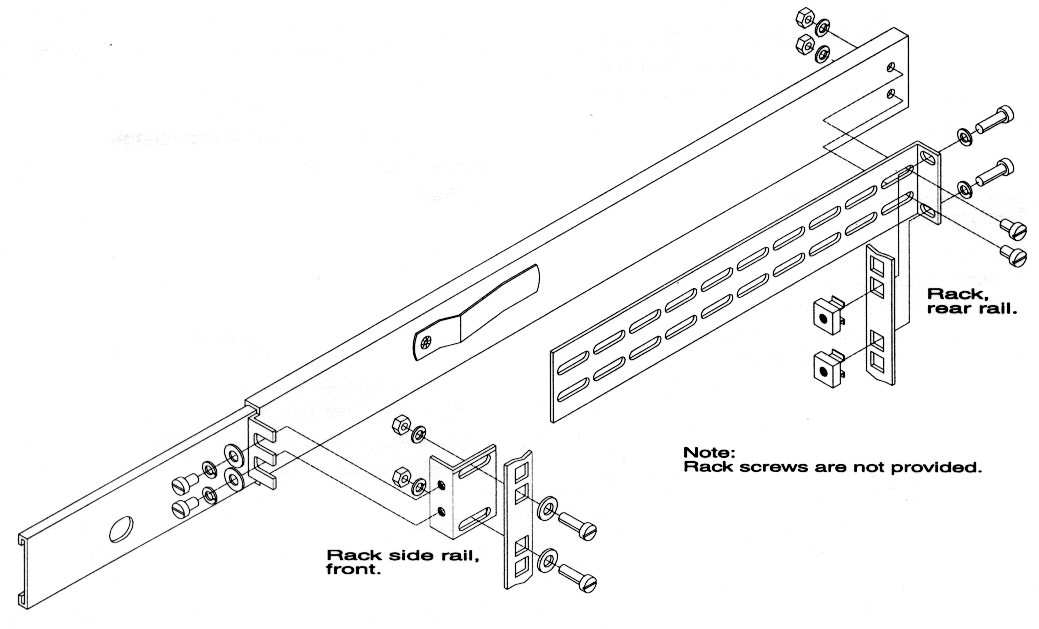
\includegraphics[width=\textwidth]{fig/rack}
\caption{Installation of PM 8552}
\end{figure}

\textbf{Removal of the Instrument}

Be sure that all cabling is disconnected before removing the instrument.
\begin{enumerate}
\item Loosen the screws in the rack frame and pull the instrument forward until the stop latches snap into their holes.
\item Press the stop latches and remove the instrument.
\end{enumerate}

\subsection{Cleaning}
\begin{itemize}
\item Disconnect the instrument from the mains voltage supply before cleaning
\item Use only a damp cloth
\item Make sure that no liquid is spilled inside the instrument
\end{itemize}

\subsection{Configuration}
\subsubsection{Remote Interface}
Move cable from connector SER (XR1) to PAR (XM1) on Main Board (Unit 1) to change from standard RS232 to simple ground-closure.

\begin{figure}[hbt]
\centering
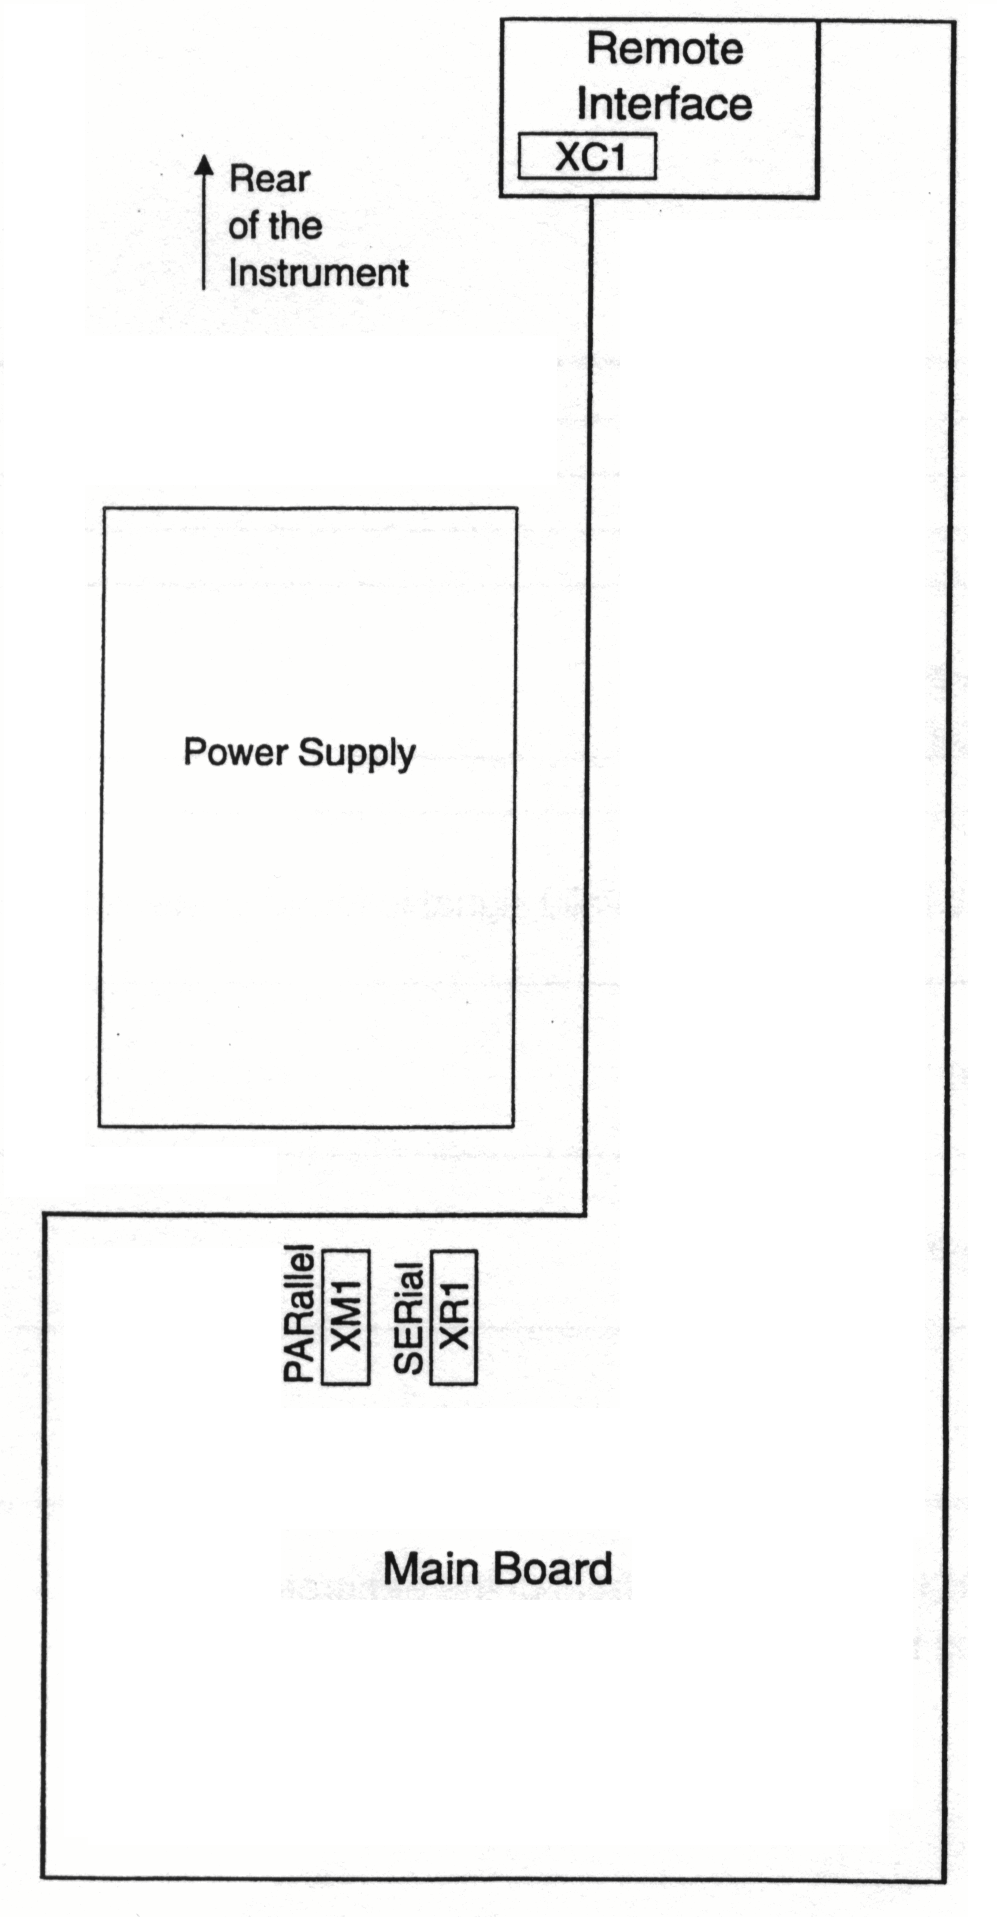
\includegraphics[width=0.5\textwidth]{fig/PT5300_overview}
\caption{Location of Connectors SER and PAR}
\label{serialconnector}
\end{figure}

\subsection{Access to and Replacement of Parts}
\subsubsection{Safety}
The opening of covers or removal of parts, expect those to which access can be gained by hand, is liable to expose live parts.

The instrument must be disconnected from all voltage sources before performing any adjustment, replacement, maintenance, or repair, which requires the instrument to be opened. If repair of the opened instrument is unavoidable, it must only be carried out by a skilled person who is aware of the hazards involved. To guarantee safety only original spare parts must be used.

\subsubsection{Access to the Units}
To gain access to the units, remove the screws that secure the top cover of the instrument and lift the cover up.

\subsubsection{Installation of Options}
The installation instruction is supplied with the option.